To generate a TikZ LaTeX code for the Hasse diagrams of a lattice \( P \) and its corresponding interval lattice \( \text{Int}\,P \), we need to understand the structure of these lattices. However, since the exact structure of \( P \) is not provided, I will create a general example of a Hasse diagram for a lattice \( P \) and its interval lattice \( \text{Int}\,P \).

Here's an example using a simple lattice \( P \):

```latex
\documentclass{standalone}
\usepackage{tikz}

\begin{document}

% Define the lattice P
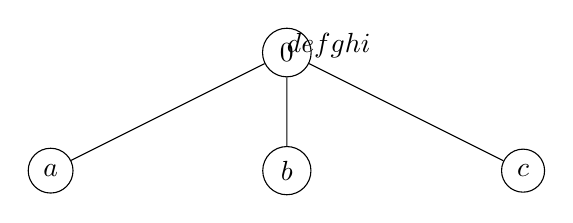
\begin{tikzpicture}[level distance=1.5cm,
  level 1/.style={sibling distance=3cm},
  level 2/.style={sibling distance=2cm},
  level 3/.style={sibling distance=1cm}]
  \node (0) [circle, draw] {0}
    child {node (a) [circle, draw] {$a$}}
    child {node (b) [circle, draw] {$b$}}
    child {node (c) [circle, draw] {$c$}};
  node (d) [circle, draw, below of=a] {$d$}
    child {node (e) [circle, draw] {$e$}}
    child {node (f) [circle, draw] {$f$}};
  node (g) [circle, draw, below of=b] {$g$}
    child {node (h) [circle, draw] {$h$}};
  node (i) [circle, draw, below of=c] {$i$};
\end{tikzpicture}

% Define the interval lattice Int(P)
\begin{tikzpicture}[level distance=1.5cm,
  level 1/.style={sibling distance=3cm},
  level 2/.style={sibling distance=2cm},
  level 3/.style={sibling distance=1cm}]
  \node (0) [circle, draw] {0}
    child {node (a) [circle, draw] {$a$}}
    child {node (b) [circle, draw] {$b$}}
    child {node (c) [circle, draw] {$c$}};
  node (d) [circle, draw, below of=a] {$d$}
    child